\documentclass{article}
\usepackage[utf8]{inputenc}
\usepackage{amsmath}
\usepackage{amssymb}
\usepackage{amsthm}
\usepackage{cancel}
\usepackage[shortlabels]{enumitem}
\usepackage{caption}
\usepackage{graphicx}
\usepackage[top=0.5in, bottom=0.5in, left=1in, right=1in]{geometry}
\usepackage{float}

% \usepackage{titlesec}
%     \titlespacing{\subsection}{\parindent}{15pt}{12pt}

\title{\textbf{\underline{MATH3090U: Netwrok Science}\\Assignment 3}}
\author{Syed Naqvi\\100590852}
\date{\today}

\begin{document}

    \maketitle
    
    \subsection*{1.}
    
    \begin{center}
        \begin{minipage}[t]{0.9\textwidth}
            I will begin by recreating the given graph using networkx:
            \begin{figure}[H]
                \centering
                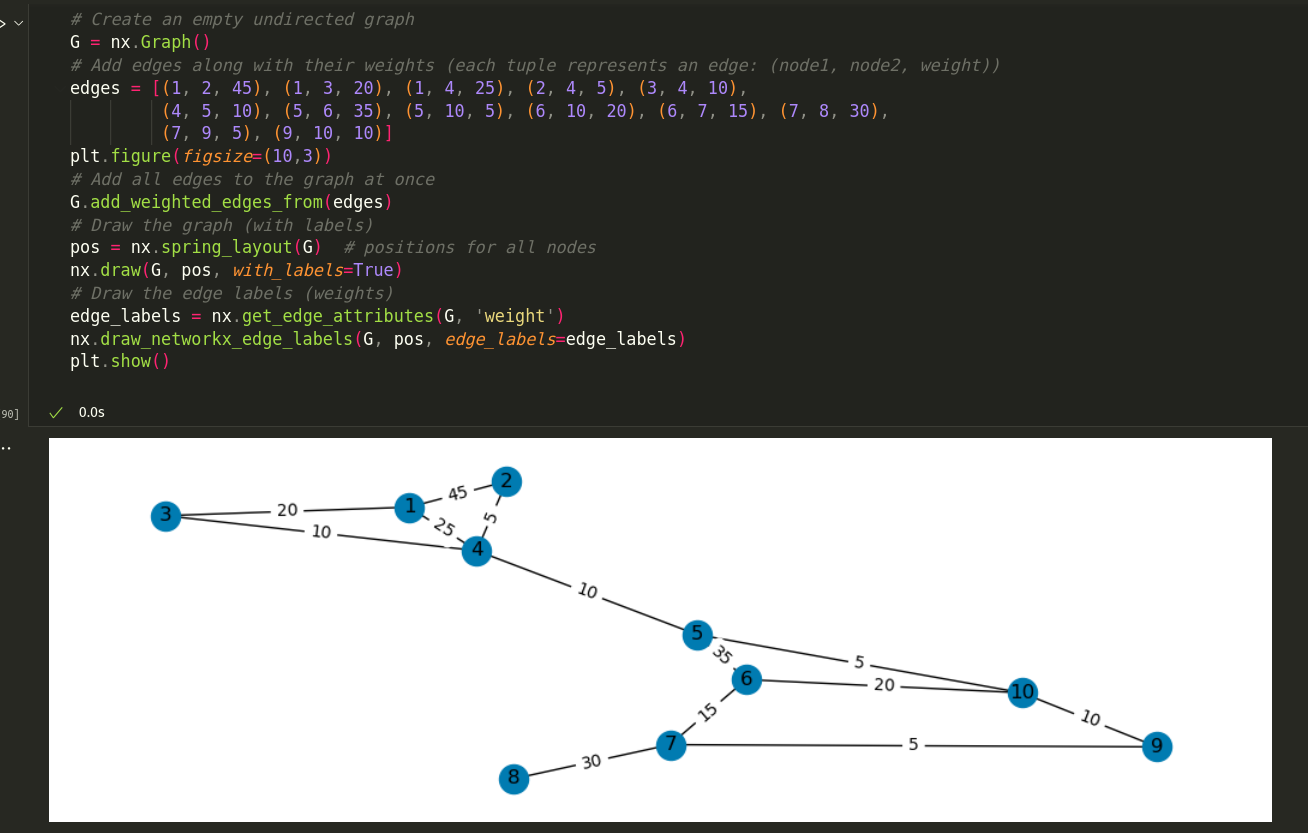
\includegraphics[width=1\textwidth, height=0.5\textheight]{./1.png}
            \end{figure}
        \end{minipage}
    \end{center}

    \begin{enumerate}[label=(\alph*), left=10pt, itemsep=10pt]
        
        \item \begin{minipage}[t]{0.9\textwidth}
            The strength of a node in this network represents the total time a child
            has spent in close contact with other children.
        \end{minipage}
        
        \item \begin{minipage}[t]{0.9\textwidth}
            The node with the maximum strength is node 1 with a total incident edge
            weigth of 90.\\
            The node with the minimum strength is node 9 with total incident edge
            weight of 15.
            \begin{figure}[H]
                \centering
                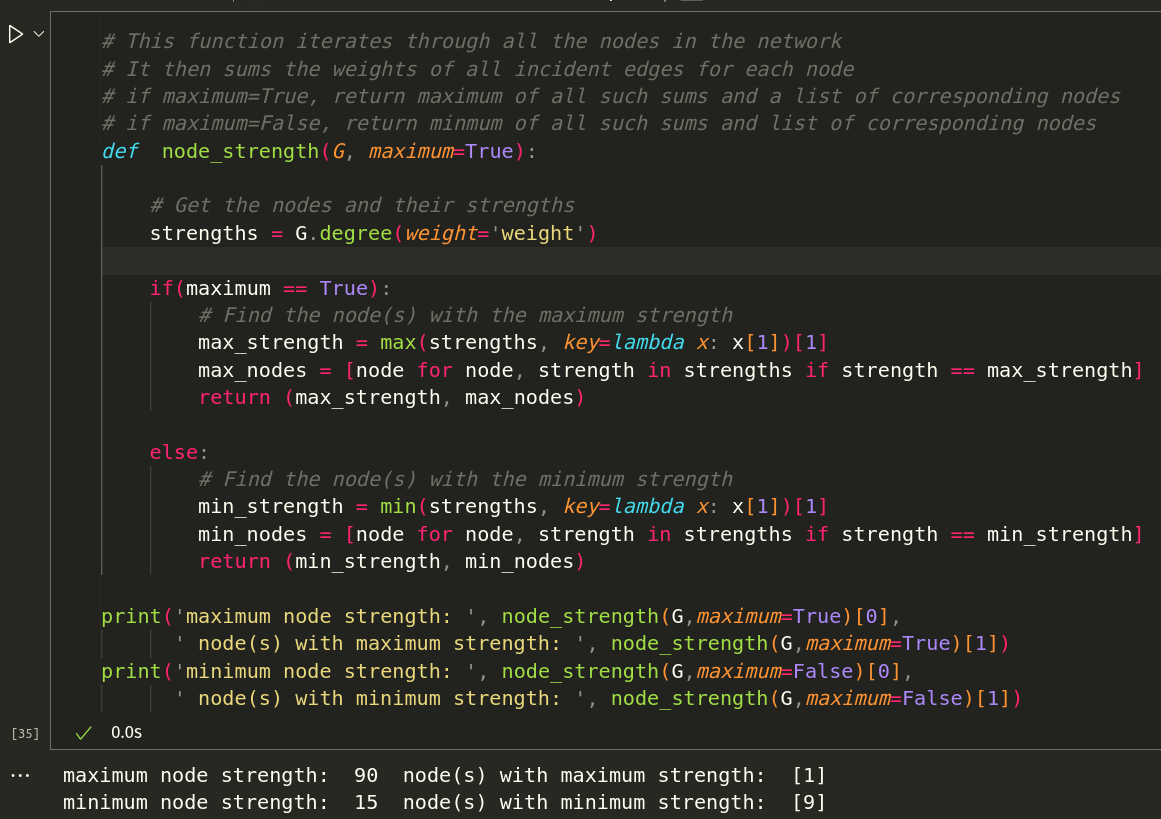
\includegraphics[width=1\textwidth, height=0.5\textheight]{./1b.png}
            \end{figure}
        \end{minipage}

        \item \begin{minipage}[t]{0.9\textwidth}
            \textbf{I disagree with this statement.}\\
            If we conclude that the highest node strength indicates the
            individual with the highest chance of getting sick then we are
            assuming that total time spent with others is the biggest risk
            factor in catching an illness. However, I would argue that it is
            not the total time spent with other people, but the actual
            \textbf{number} of different people with whom the time is being
            spent that is the biggest risk factor as this increases possible
            exposures to the illness.
            
            That being said, the raw node strength does not indicate the amount
            of different people (possible carriers of a sickness) an
            individual has been in close contact with since
            a high node strength could mean lots of time spent with a single
            person or little time spent with many people. Take the example of
            node 1 with node strength 90 and node 4 with node strength 50. Node
            4 has a much lower node strength than node 1 yet has a higher
            unweighted degree meaning the child represented by node 4 has
            had more opportunities than the child represented by node 1 to catch
            the sickness from other children.  
        \end{minipage}

        \item \begin{minipage}[t]{0.9\textwidth}
            We can use networkx to calculate the closeness centrality of all nodes diregarding weights:
            \begin{figure}[H]
                \centering
                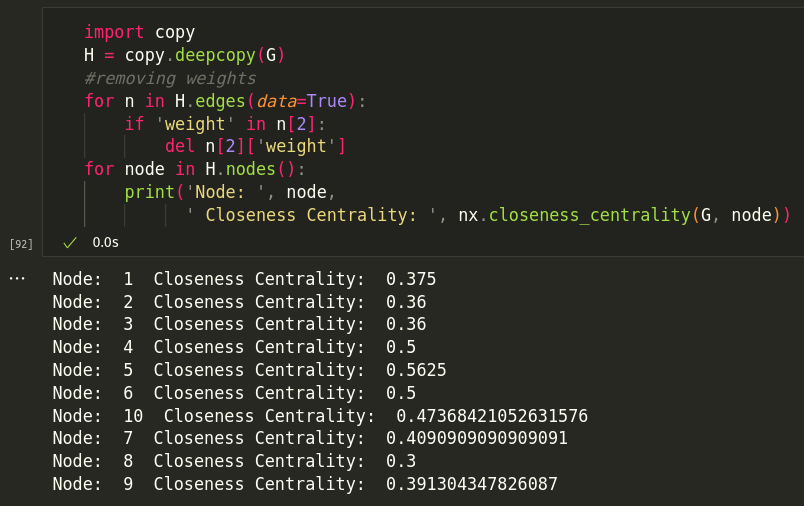
\includegraphics[width=1\textwidth, height=0.3\textheight]{./1d.png}
            \end{figure}
        \end{minipage}

        \item \begin{minipage}[t]{0.9\textwidth}
            The path of fewest edges between nodes 3 and 5 is the sequence 3, 4, 5, 6. The weighted distance of
            this path is the sum of the weights of each edge in the sequence 10 + 10 + 35 = 55.\\
            $\therefore$ the weighted distance of the path of fewest edges between nodes 3 and 6 is 55.
        \end{minipage}

        \item \begin{minipage}[t]{0.9\textwidth}
            The path with fewest edges between nodes 3 and 6 is P = [3, 4, 5, 6] with a total weight of 55.
            If we interpret weight as the length of an edge then the path Q = [3, 4, 5, 10, 6] has more edges but
            has a total distance (sum of all path lengths) of 45 which is less than 55 and so we would say that
            Q has a shorter length than P.
        \end{minipage}

        \item \begin{minipage}[t]{0.9\textwidth}
            The closeness centrailty of a node is the reciprocal of the average of the shortest paths between the given
            node and every other node in the network. Using weight of an edge as the distance between adjacent nodes means the
            shortest path is the one of least total weight instead of fewest edges. However, given that weight in our child
            network is the time two children have spent in close proximity, we can see that it is more sensible for a larger
            weight to represent a stronger relationship or higher "closeness" between two nodes. Thus, using weighted paths in
            the closeness centrality formula would actually require us to find the weakest or "least close" connections
            between two nodes, providing no inforamtion of a node's closeness to other nodes since we will have excluded the
            true closest paths from our calculations. Therefore using the weighted distance with our network's definition of
            weight in the closeness centrality formula would not be very useful.
        \end{minipage}

        \item \begin{minipage}[t]{0.9\textwidth}
            We can use networkx to create a deepcopy of our original weighted network and then set each weight
            to its reciprocal. We can then print this graph and find the shortest distance between nodes 1 and 5 in
            terms of cost as our new weight assignment:
            \begin{figure}[H]
                \centering
                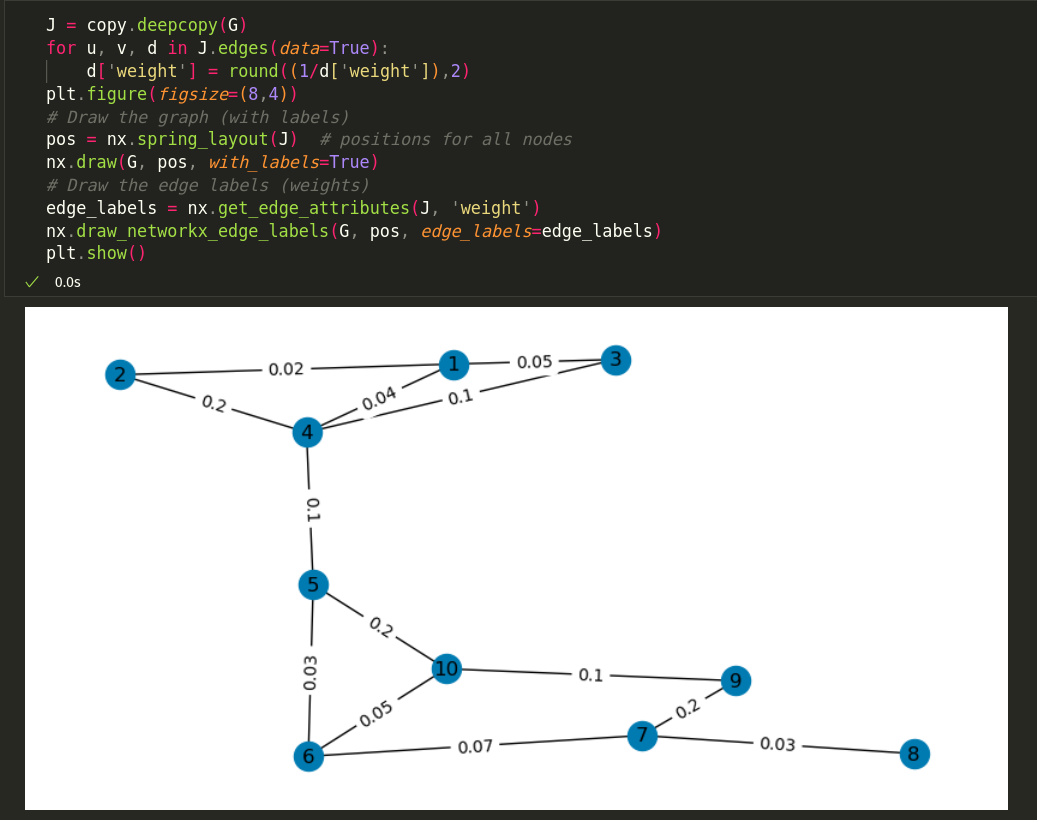
\includegraphics[width=1\textwidth, height=0.5\textheight]{./1h.png}
            \end{figure}
            As we can see from the graph, the sequence 1, 4, 5 provides a shortest distance of 0.14 between nodes
            1 and 5.
        \end{minipage}

        \item \begin{minipage}[t]{0.9\textwidth}
            Having reproduced the graph with the weights being set to their reciprocals in the previous question,
            we can now find the nodes most central by closeness centrality.
            \begin{figure}[H]
                \centering
                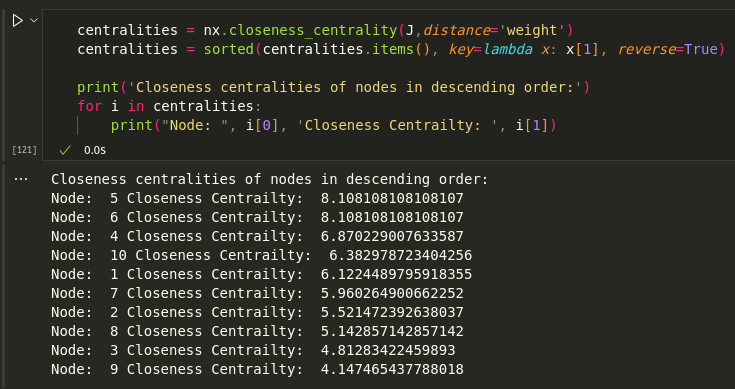
\includegraphics[width=1\textwidth, height=0.3\textheight]{./1i.png}
            \end{figure}
        \end{minipage}

        \item \begin{minipage}[t]{0.9\textwidth}
            The closeness centralities of nodes 5 and 6 are highest. This means that nodes 5 and 6 have the most paths
            of least resistance (lowest total cost, highest overall weights per edge) connecting them to every other node in
            the network. In the context of our network where total time spent with other children is the main disease spreading
            risk factor, these closeness centrailty results suggest a sickness will have the most amount of time to spread
            \textbf{from} every node in the network \textbf{to} nodes 5 and 6 as well as \textbf{from} nodes 5 and 6 \textbf{to}
            every other node in the network. This is due to interaction times being longest between nodes along paths where nodes
            5 or 6 are endpoints.
        \end{minipage}

    \end{enumerate}


    \subsection*{2.}

    \begin{enumerate}[label=(\alph*), left=10pt, itemsep=10pt]
        \item \begin{minipage}[t]{0.9\textwidth}
            Suppose we are given two degree sequences to apply to a network $G$ where $|V(G)| = n$ and initially,
            $|E(G)| = 0$. The first sequence $I = [a_{1}, a_{2}, \dots a_{k}]$ consisits of $indegrees$ while the second sequence
            $O = [b_{1}, b_{2}, \dots b_{r}]$ consists of $outdegrees$.\\
            
            First we go through our network $G$ and arbitrarily select nodes $n_{i}$, $n_{j} \in G$ where it may or may not
            be the case that $n_{i} = n_{j}$. We attach $a_{i}$ inward-directed half-edges to $n_{i}$ and $b_{j}$
            outward-directed half-edges to $n_{j}$. Once this process is complete, there will always exist nodes $n_{i}$,
            $n_{j} \in G$ such that $\forall a_{i} \in I$ and $\forall b_{j} \in O$, $indegree(n_{i}) = a_{i}$ and
            $outdegree(n_{j}) = b_{j}$.\\
            
            Next, we arbitrarily connect the outward-directed half-edges to the inward-directed half-edges until there are
            no more half-edges remaining. This leaves us with a random directed graph, generated using an adaptation of
            the configuration model. Note that this process permits the existence of un-conneceted nodes, self-loops and
            multi-edges.\\

            We know that for directed graphs, the total $indegree$ must equal the total $outdegree$. This means that degree
            sequences $I$ and $O$ should be defined so that $\sum_{i}^{k} a_{i} = \sum_{j}^{r}b_{j}$ as this will ensure all
            inward-directed half-edges have a corresponding outward-directed half-edge, leaving no "dangling" edges.
            Another requirement that must be met for this algorithm to work is that $n \geq max(|I|,|O|)$. This is so that
            there are enough nodes to which we can apply all the degrees in the lengthier of sequences $I$ and $O$.  

        \end{minipage}
    \end{enumerate}

    \subsection*{3.}

    \begin{center}
        \begin{minipage}[t]{0.9\textwidth}
            First we create 100 $G(n,p)$ graphs with $n=60$ and $p=(1/25)$. We then calculate the required graph statistics
            for each graph and store the values in a list for later analysis.
            \begin{figure}[H]
                \centering
                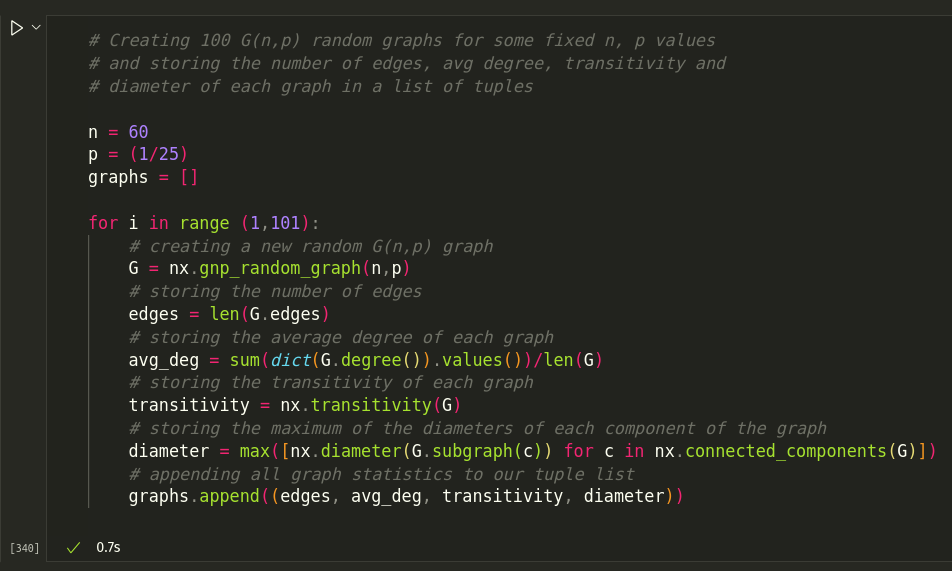
\includegraphics[width=1\textwidth, height=0.3\textheight]{./3.png}
            \end{figure}
        \end{minipage}
    \end{center}

    \begin{enumerate}[label=(\alph*), left=10pt, itemsep=10pt]
        \item \begin{minipage}[t]{0.9\textwidth}
            Comparing the average values with each parameter we see that they are almost identical. The expected diameter
            is also of the correct order of magnitude.
            \begin{figure}[H]
                \centering
                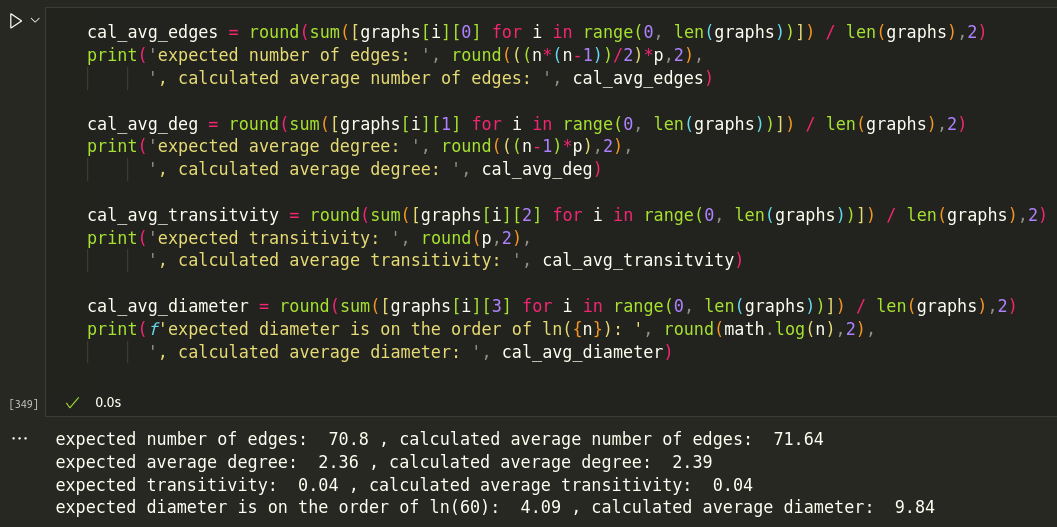
\includegraphics[width=1\textwidth, height=0.3\textheight]{./3a.png}
            \end{figure}
        \end{minipage}
        
        \item \begin{minipage}[t]{0.9\textwidth}
            We can see that the number of edges and the average degree are both roughly normally distributed, with most
            graphs having average degree and number of edges near our earlier calculated values. As we move towards the tails,
            there are fewer graphs. 
            \begin{figure}[H]
                \centering
                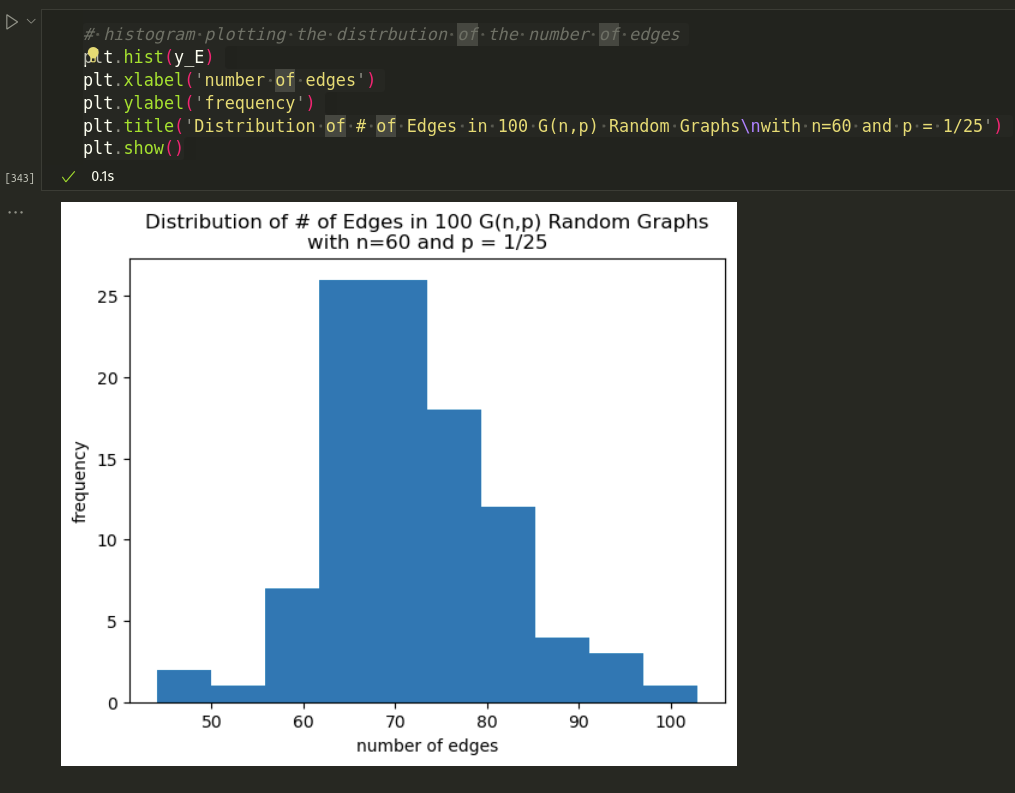
\includegraphics[width=1\textwidth, height=0.4\textheight]{./3bi.png}
            \end{figure}
            \begin{figure}[H]
                \centering
                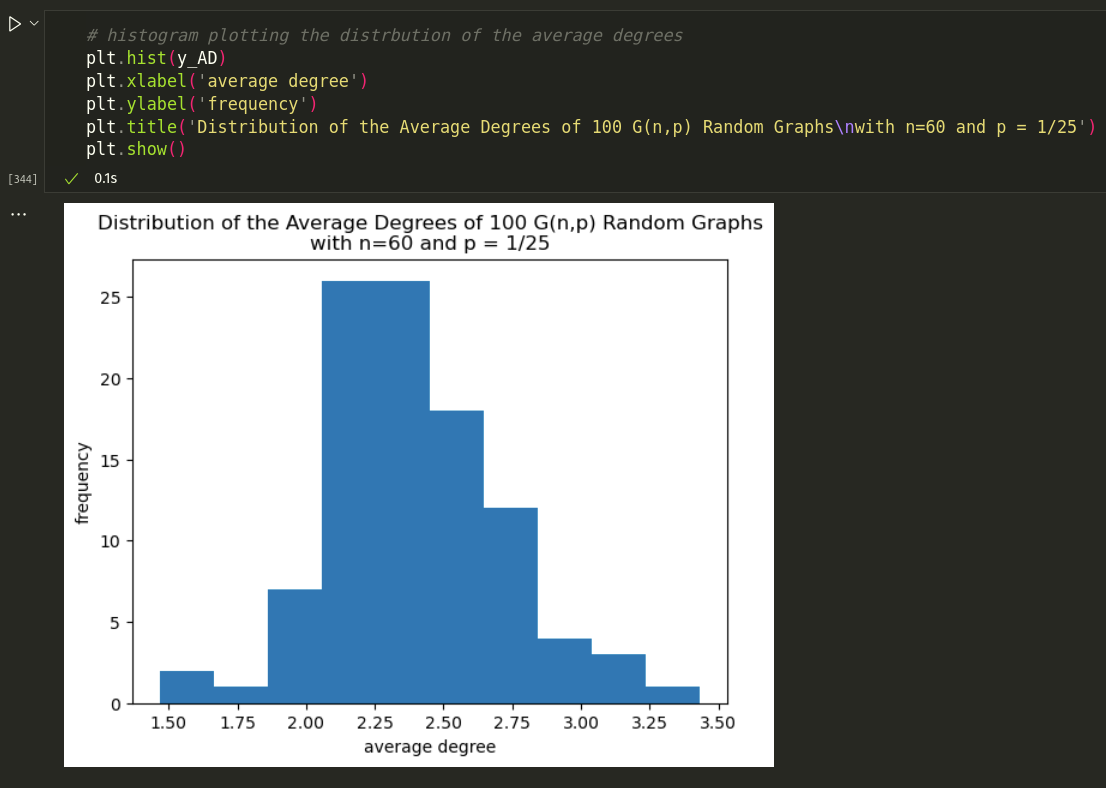
\includegraphics[width=1\textwidth, height=0.4\textheight]{./3bii.png}
            \end{figure}
        \end{minipage}
        \newpage
        \begin{minipage}[t]{0.9\textwidth}
            The distribution of transitivities exists within a range of 0 to just above 0.1 indicating that the probabiltiy
            of forming trinagles within these graphs is relatively low which makes sense given the low p value. The graph is
            right skewed suggesting that the number of graphs decreases as the transitivity increases. This is again as expected
            because the probability of there being an edge between \textbf{any} pair of nodes, let alone those with a common neighbor
            is low: 1/25. We can also see that there is a large number of graphs with a transitivity around 0.2 to 0.4 which
            does roughly align with our calculated and expected transitivity averges of 0.4. 
            \begin{figure}[H]
                \centering
                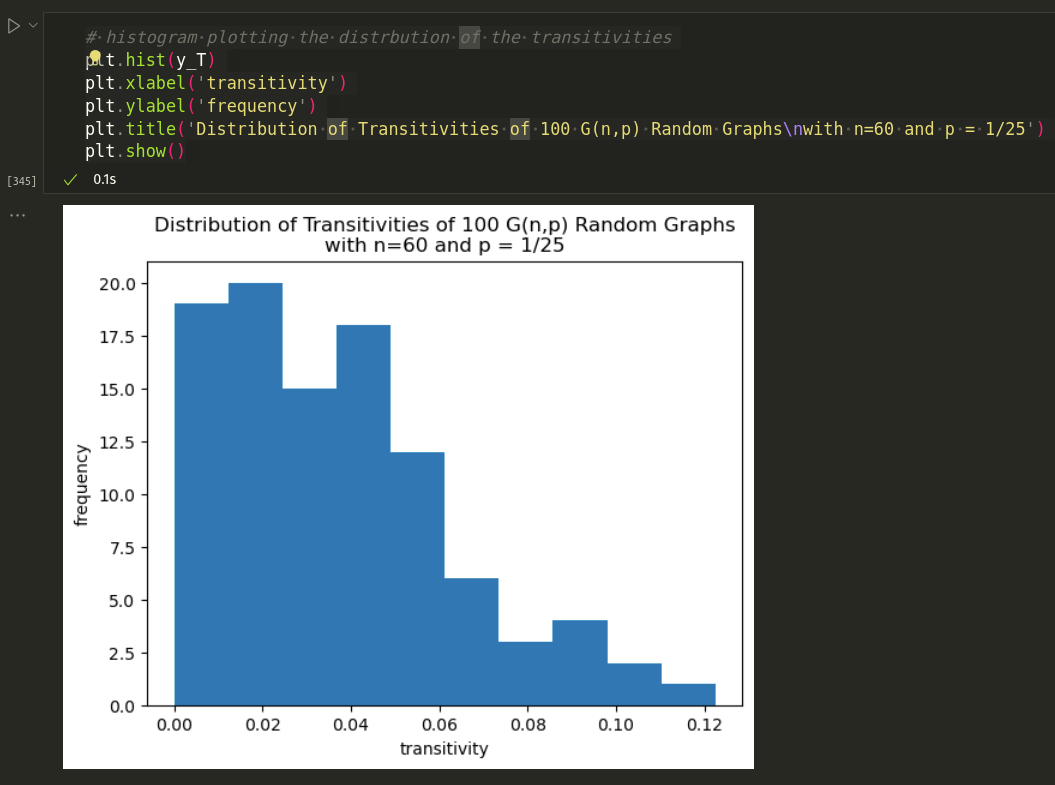
\includegraphics[width=1\textwidth, height=0.35\textheight]{./3biii.png}
            \end{figure}
            By convention, we considered the largest of the diameters of each connected component as the diameter of
            the random graphs. With this definition, we see that the diameter distribution seems roughly normally distributed,
            with a slightly right skew. It seems that the majority of the random graphs had a diameter close to 10 with a
            non-insignificant amount having diameter above above 10. This shows the random nature of the graphs and
            the rough diameter predition being on the order of ln(n) which these results do seem to to demonstrate.  
            \begin{figure}[H]
                \centering
                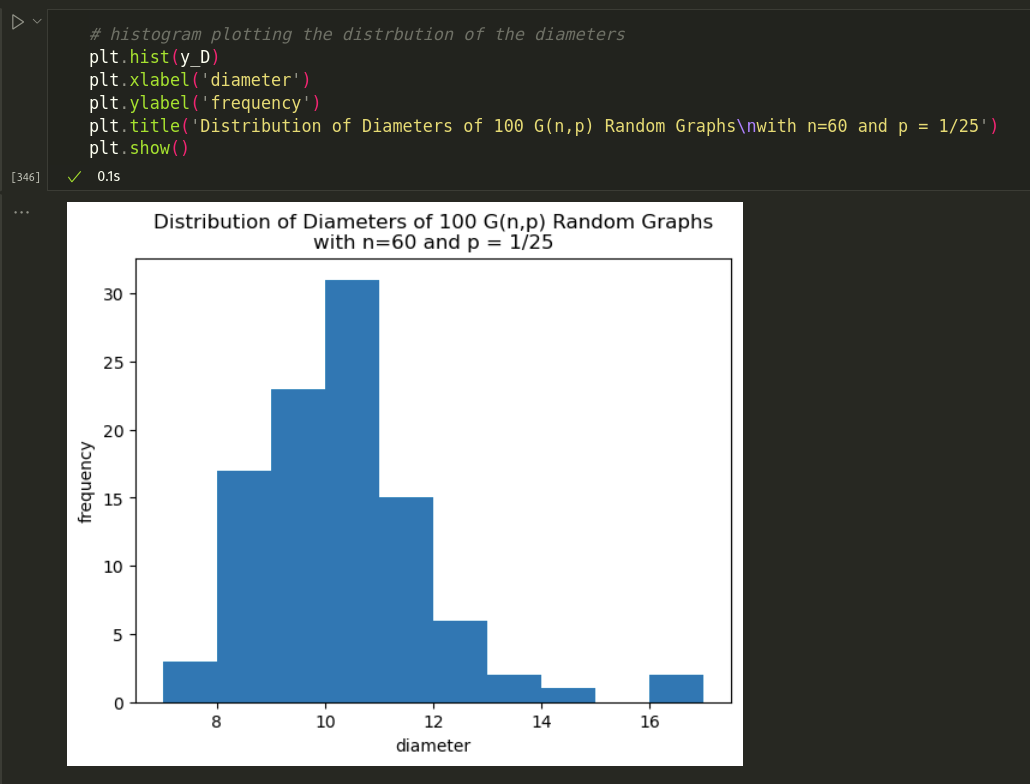
\includegraphics[width=1\textwidth, height=0.35\textheight]{./3biv.png}
            \end{figure}
        \end{minipage}

    \end{enumerate}
\end{document}